%
% Systemen voor Online Verkiezingen
% @author Pieter Maene <pieter.maene@student.kuleuven.be>
%

\documentclass[master=elt,masteroption=im,inputenc=utf8]{kulemt}
\setup{title={Online verkiezingen in de praktijk: verbetering en toepassing van het Helios verkiezingssysteem},
  author={Pieter Maene},
  promotor={Prof. dr. ir. Bart Preneel},
  assessor={Prof. dr. ir. V. Rijmen \and Prof. dr. ir. L. Van Eycken},
  assistant={Dr. ir. J. Hermans \and Dr. ir. F. Vercauteren}
}

\setup{filingcard,
  translatedtitle={Online Elections in Practice: Improvement and Application of the Helios Voting System},
  udc=621.3,
  shortabstract={
    %
% Short Abstract
% @author Pieter Maene <pieter.maene@student.kuleuven.be>
%

Een voter-verifiable stemsysteem geeft de kiezer de mogelijkheid om na te gaan of zijn eigen stem correct geregistreerd is en of het resultaat correct is. Het is mogelijk om een dergelijk systeem met papieren stembiljetten te implementeren, zowel met als zonder cryptografische technieken. Helios is een voter-verifiable stemsysteem voor online verkiezingen. De procedure die bij deze systemen gevolgd moet worden, is echter vaak zeer complex. In deze thesis wordt de procedure gegeven die in Helios gevolgd moet worden om een verkiezing op te zetten. De interface van het systeem werd ook herwerkt om de beheerder beter te ondersteunen. Ook de applicatie die gebruikt wordt door de kiezers werd vereenvoudigd. Na het systeem uitgebreid getest te hebben, werd het in de praktijk gebruikt voor een re\"ele verkiezing waarbij ongeveer 750 mensen hun stem uitbrachten. Daarnaast wordt besproken hoe de trustees hun geheime sleutels kunnen bewaren. Er wordt ook onderzocht of de tekstuele fingerprints niet op een betere manier weergegeven kunnen worden. Tot slot worden de prestaties van de Web Cryptography API vergeleken met deze van bestaande implementaties in JavaScript. Deze nieuwe specificatie geeft ontwikkelaars toegang tot cryptografische functies die in de browser ingebouwd zijn.
  }
}

% Font
\setup{font=lm}

% Packages
\usepackage{amsmath,amssymb,mathtools}
\usepackage{color}
\usepackage{float}
\usepackage{kulemtx}
\usepackage{multirow,bigstrut}
\usepackage[np,autolanguage]{numprint}
\usepackage{pdfpages}
\usepackage{tikz}
\usepackage{url}

% The "colorlinks" option should be removed for the print version
\usepackage[pdfusetitle,plainpages=false]{hyperref}

% Remove the "%" on the next line to print the cover
%\setup{coverpageonly}

% Customisations
\graphicspath{{./images/}}
\usetikzlibrary{arrows,fit,shapes}
\setlength{\parindent}{0pt}
\headstyles{kulemtman}

% Document
\begin{document}

  % Alias
  %
% Alias
% @author Pieter Maene <pieter.maene@student.kuleuven.be>
%

\renewcommand{\ref}[1]{\mbox{\autoref{#1}}}

\renewcommand{\chapterautorefname}{Chapter}
\renewcommand{\equationautorefname}{Eq.}
\renewcommand{\figureautorefname}{Fig.}
\renewcommand{\footnoteautorefname}{Footnote}
\renewcommand{\itemautorefname}{Item}
\renewcommand{\sectionautorefname}{Section}
\renewcommand{\subsectionautorefname}{Section}
\renewcommand{\subsubsectionautorefname}{Section}
\renewcommand{\paragraphautorefname}{Paragraph}
\renewcommand{\subparagraphautorefname}{Paragraph}
\renewcommand{\pageautorefname}{Page}
\renewcommand{\tableautorefname}{Table}

\newcommand{\cplusplus}{C\texttt{++}\ }
  % 
% TikZ
% @author Pieter Maene <pieter.maene@student.kuleuven.be>
%

\tikzstyle{decision} = [diamond, draw, fill=black!20, text width=4.5em, text badly centered, node distance=3cm, inner sep=0pt]
\tikzstyle{block} = [rectangle, draw, fill=black!20, text width=5em, text centered, rounded corners, minimum height=4em]
\tikzstyle{line} = [draw, -latex']

  \begin{preface}
    % 
% Preface
% @author Pieter Maene <pieter.maene@student.kuleuven.be>
%

%TODO Voorwoord
  \end{preface}

  \kulemtmanToC
  \tableofcontents

  \begin{abstract}
    % 
% Abstract
% @author Pieter Maene <pieter.maene@student.kuleuven.be>
%

Verkiezingen spelen een belangrijke rol in een democratische maatschappij. Kiezers moeten op een betrouwbare en gebruiksvriendelijke manier hun stem kunnen uitbrengen. Bij de huidige systemen moet de kiezer vertrouwen hebben in de organisatie die verantwoordelijk is voor de verkiezingen. Een voter-verifiable stemsysteem geeft de kiezer de mogelijkheid om na te gaan of zijn eigen stem correct geregistreerd is en of het resultaat correct is.

\npar Het is mogelijk om een dergelijk systeem met papieren stembiljetten te implementeren, zowel met als zonder cryptografische technieken. Helios is een voter-verifiable stemsysteem voor online verkiezingen. De procedure die bij deze systemen gevolgd moet worden, is echter vaak zeer complex.

\npar In deze thesis wordt de procedure gegeven die in Helios gevolgd moet worden om een verkiezing op te zetten. De interface van het systeem werd ook herwerkt om de beheerder beter te ondersteunen. Ook de applicatie die gebruikt wordt door de kiezers werd vereenvoudigd. Na het systeem uitgebreid getest te hebben, werd het in de praktijk gebruikt voor een re\"ele verkiezing waarbij ongeveer 750 mensen hun stem uitbrachten.

\npar Daarnaast wordt besproken hoe de trustees hun geheime sleutels kunnen bewaren. Er wordt ook onderzocht of de fingerprints waarvoor momenteel strings gebruikt worden niet op een betere manier weergegeven kunnen worden. Tot slot worden de prestaties van de Web Cryptography API vergeleken met deze van bestaande implementaties in JavaScript. Deze nieuwe specificatie geeft ontwikkelaars toegang tot cryptografische functies die in de browser ingebouwd zijn.
  \end{abstract}
  
  \listoffiguresandtables
  
  \chapter{Lijst van afkortingen en symbolen}
  \section*{Lijst van afkortingen}
  \begin{flushleft}
    \renewcommand{\arraystretch}{1.1}
    \begin{tabularx}{\textwidth}{@{}p{14mm}X@{}}
      API & Application Programming Interface \\
      DRE & Direct-Recording Electronic \\
      SBA & Short Ballot Assumption \\
      VVPAT & Voter-Verified Paper Audit Trail
    \end{tabularx}
  \end{flushleft}
  \section*{Lijst van symbolen}
  \begin{flushleft}
    \renewcommand{\arraystretch}{1.1}
    \begin{tabularx}{\textwidth}{@{}p{14mm}X@{}}
      $pk$ & Publieke sleutel \\
      $sk$ & Geheime sleutel \\
      $df$ & Decryptiefactor
    \end{tabularx}
  \end{flushleft}

  \mainmatter

  % Chapters
  \include{chapters/03-inleiding}
  
  %
% Literatuurstudie
% @author Pieter Maene <pieter.maene@student.kuleuven.be>
%

\chapter{Literatuurstudie}
\label{chap:literatuurstudie}

Deze thesis handelt over methoden voor online verkiezingen. Een interessant verwant probleem zijn systemen die gebruik maken van papier. In dit hoofdstuk wordt specifiek gekeken naar papieren voter-verifiable systemen.

\npar In \ref{sec:ls:geschiedenis} wordt eerst een kort overzicht van de geschiedenis van stemsystemen gegeven. Vervolgens worden de voornaamste vereisten bekeken waaraan deze systemen moeten voldoen (\ref{sec:ls:vereisten}). Belangrijk hierbij is de definitie van een voter-verifiable systeem. Tot slot worden zowel systemen onderzocht die geen gebruik maken van cryptografische methoden (\ref{sec:ls:systemen_zonder_cryptografie}) als deze die daar wel op steunen (\ref{sec:ls:systemen_met_cryptografie}).

\section[Geschiedenis]{Geschiedenis~\cite{adida_advances_in_cryptographic_voting_systems}}
\label{sec:ls:geschiedenis}

Onze samenleving heeft een rijke geschiedenis van stemprocedures, die teruggaat tot Athene in het oude Griekenland. Hier bracht men een negatieve stem uit op een potscherf. In deze paragraaf bekijken we kort enkele methodes die bepalend zijn geweest voor de manier waarop we vandaag werken.\cite{wiki:ostracon}

\npar Sinds de uitvinding van het geheime stembiljet in 1858 in Australi\"e, is er eigenlijk niet meer zoveel veranderd. In dit systeem worden de biljetten op voorhand gedrukt door de staat en veilig bewaard tot op de stemdag. Elke stemgerechtigde krijgt op de stemdag een biljet waarna hij zijn stem uitbrengt in een stemhokje. Het grootste voordeel van deze methode ligt in het feit dat elke stem geheim is.

\npar Deze stemmethode maakte het daarnaast ook mogelijk om mechanische (en later elektrische) machines te gebruiken. Mechanische systemen werden gebruikt in grotere gemeenschappen en waren gebaseerd op hendels en mechanische tellers. De eerste van deze machines werd in 1892 ingevoerd in New York. Rond 1960 werden de eerste elektrische machines ingevoerd. Deze maakten gebruiken van optische scans. Bij deze systemen moest de stem meestal op een specifieke manier aangegeven worden, bijvoorbeeld door het inkleuren van bolletjes.

\npar Sinds 2000 worden steeds vaker DRE machines gebruikt. Hierop draait speciale stemsoftware die de keuze van de kiezer digitaal vastlegt. Deze machines maken het stemproces aanzienlijk eenvoudiger. Het grootste probleem is dat de kiezer geen enkele bevestiging krijgt en dat hij deze machines dus volledig moet vertrouwen.\cite{wiki:dre_voting_machine}

\npar Het gebrek aan controle door de kiezer bij DRE vormde de aanleiding voor het ontwerpen van VVPAT machines. Hierbij toont de machine de kiezer een afgeschermde afdruk van zijn stem, waarna hij deze kan accepteren of weigeren. Op die manier kan de kiezer verifi\"eren of zijn stem correct is. In principe zouden bij een hertelling dan ook deze papieren tickets en niet de digitale data gebruikt moeten worden.\cite{mercuri_voting_machine_risks}

\section{Vereisten}
\label{sec:ls:vereisten}

Bij het ontwerpen van een stemsysteem zijn er twee tegenstrijdige doelen. Enerzijds moet het mogelijk zijn dat de kiezer thuis kan controleren of zijn stem juist meegeteld is. Anderzijds mag diezelfde persoon niet kunnen bewijzen voor wie hij precies gestemd heeft, noch mag het mogelijk zijn dat anderen hierachter kunnen komen. Wanneer hij dit wel kan, zou hij zijn stem kunnen verkopen aan iemand die de verkiezing wil beïnvloeden of gedwongen kunnen worden om op een bepaalde kandidaat te stemmen.

\npar Hoewel het vaak zeer moeilijk is om een grote verkiezing doorslaggevend te wijzigen, wordt stemfraude toch regelmatig geconstateerd.\cite{adida_advances_in_cryptographic_voting_systems} E\'en van de grote moeilijkheden is dat zowel kiezers als bijzitters corrupt kunnen zijn. Er kan van geen enkele deelnemer verwacht worden dat hij eerlijk is.

\npar Het is dus essentieel dat het stemsysteem vertrouwd wordt door de kiezers. Bij de huidige systemen moet hij zijn vertrouwen echter meestal leggen bij de instantie die de verkiezing organiseert (\ref{sec:ls:vertrouwen}). Nieuwe technieken laten ons echter toe om \textit{end-to-end} verifiable systemen te ontwikkelen, waar de kiezer zelf de correctheid van het resultaat kan nagaan (\ref{sec:ls:end_to_end_verifiability}).

\subsection{Vertrouwen}
\label{sec:ls:vertrouwen}

De huidige manier van stemmen vereist dat de kiezer zeer veel vertrouwen legt in het gebruikte systeem. Zoals verder besproken wordt (\ref{sec:ls:end_to_end_verifiability}), zijn er nieuwe ontwerpen waarbij de kiezer kan controleren of zijn stem correct meegeteld is. Deze systemen steunen vaak op moeilijke cryptografische technieken, die heel wat achtergrondkennis vragen om ze te begrijpen.

\npar Een vereiste voor om het even welk stemsysteem is dat het vertrouwd wordt door een gemiddelde kiezer, de bijzitters, de publieke opinie en media. Opdat deze mensen een dergelijk systeem zouden vertrouwen, moeten de experts die het systeem goedkeuren dit op een eenvoudige manier aan hen kunnen uitleggen.\cite{randell_ryan_voting_technologies_and_trust} Daarom zullen eenvoudige systemen die geen gebruik maken van cryptografie, waarschijnlijk sneller aanvaard worden door een breed publiek.

\subsection{End-to-End Verifiability}
\label{sec:ls:end_to_end_verifiability}

In een end-to-end verifiable voting systeem wordt niet nagegaan of de code van de stemmachines volledig correct is. In plaats daarvan wordt wiskundig bewezen dat het resultaat correct is. Op die manier kan de moeilijke en vaak ondoorzichtige fysische \textit{chain of custody} vermeden worden. Dit betekent ook dat iemand niet langer speciale toegang moet hebben om de resultaten te controleren. Om het even wie kan nagaan of de bewijzen correct zijn.

\npar Dergelijke systemen kunnen zowel met als zonder cryptografische technieken gerealiseerd worden. Cryptografie kan enerzijds gebruikt worden om stemmen te encrypteren, zodat ze zeker geheim blijven. Anderzijds geven sommige systemen een \textit{zero-knowledge} bewijs dat aantoont dat de stemmen correct geteld zijn.

\section{Systemen zonder cryptografie}
\label{sec:ls:systemen_zonder_cryptografie}

In deze paragraaf worden enkele systemen besproken waarin geen gebruik gemaakt wordt van cryptografie. Open Counting (\ref{sec:ls:open_counting}) is een techniek waarbij alleen de telfase aangepast wordt. Floating receipts (\ref{sec:ls:floating_receipts}) kunnen de veiligheid van elk papieren stemsysteem sterk verbeteren. ThreeBallot (\ref{sec:ls:scratch_card}) en Scratch-Card zijn beiden voter-verifiable systemen die gebruik maken van papieren tickets. Twin (\ref{sec:ls:twin}) bouwt verder op floating receipts. Vooral ThreeBallot wordt in detail besproken omdat de belangrijkste concepten van papier-gebaseerde voter-verifiable verkiezingen hierin aan bod komen.

\subsection[Open Counting]{Open Counting~\cite{adi_schuler_frohlich_open_counting}}
\label{sec:ls:open_counting}

Open counting vertrekt van de systemen zoals we ze vandaag kennen, maar de stemmen worden op een nieuwe manier geteld. Het stembiljet is aangepast om eenvoudig optisch geteld te worden. De stemmen worden nog steeds geteld door ambtenaren. Elke stem wordt op een scherm getoond aan verschillende telstations, elk met hun eigen hardware die het getoonde biljet filmt en analyseert. Ieder station geeft op regelmatige tijdstippen zijn huidig totaal en wanneer er onenigheid is, wordt het gedisputeerde biljet gezocht en het probleem opgelost.

\npar Tijdens het tellen geeft ieder station ook een hash van hun opgenomen video. Hiervoor wordt een veilige hash-functie gebruikt. Deze hashes kunnen dan later aangewend worden tijdens een geautomatiseerde audit om te controleren of er niet geknoeid is met de beelden. Dit proces is publiek en dus kan iedereen zijn eigen hardware meebrengen en de telling zelf uitvoeren. Het systeem wordt zo ontworpen dat een eenvoudige camera en computer volstaan. Ook deze waarnemers kunnen een hash van hun video publiceren om geloofwaardiger over te komen.

\npar De verschillende telstations controleren continu elkaar en ook de waarnemers kunnen achteraf onregelmatigheden melden. Omdat het systeem snel werkt, kan de telling in het stembureau zelf gehouden worden. Op die manier kunnen alle belanghebbenden aanwezig zijn en kan het transport van de ongetelde biljetten vermeden worden. Het transparante karakter en het gebruik van eenvoudige hardware kunnen het vertrouwen van de kiezers in het systeem sterk vergroten.

\npar Open counting is een relatief eenvoudige manier om de telprocedure transparanter te maken naar de kiezers. Elke stem moet echter afzonderlijk getoond worden, waardoor dit systeem alleen gebruikt kan worden wanneer het aantal biljetten beperkt is.

\subsection[Floating Receipts]{Floating Receipts~\cite{rivest_smith_three_voting_protocols}}
\label{sec:ls:floating_receipts}

Floating receipts zijn een waardevolle toevoeging voor elk voter-verifiable papieren telsysteem. Een doos met stembiljetten wordt aan de uitgang van het stembureau geplaatst. De kiezer maakt bij het buitengaan een kopie van een stembiljet dat hij hieruit trekt, vooraleer hij zijn eigen exemplaar erbij legt. Hij neemt dus een willekeurig ticket mee dat niet het zijne is, maar hij kan dit ticket toch later gebruiken om te controleren of de stemprocedure correct verlopen is. Omdat de doos initieel leeg is, krijgen de eerste $T$ kiezers geen ticket mee naar huis. Hierbij is $T$ een constante die veel kleiner is dan het aantal kiezers, maar voldoende groot zodat $1/T$ klein is.

\npar Niemand weet dus met grote waarschijnlijkheid van wie hij het biljet gekopieerd heeft. Omdat de aanvaller geen betrouwbare methode heeft om alle kopie\"en van een ticket te bemachtigen, is het systeem bestendig tegen het vervangen van biljetten of het verkopen van een stem. Een nadeel is dat de kiezer niet langer zijn eigen ticket heeft en dus misschien minder gemotiveerd is om te controleren of dit correct meegeteld is. Er wordt echter verondersteld dat een groot aantal kiezers dat toch nog steeds zal doen.

\npar Om floating receipts te gebruiken, moeten de kiezers een extra stap volgen in de stemprocedure. De stemprocedure wordt dus complexer, maar dit kan verantwoord worden door de voordelen die deze techniek met zich meebrengt.

\subsubsection{Short Ballot Assumption}
\label{sec:ls:short_ballot_assumption}

Bij de SBA moet het aantal kandidaten op het biljet beperkt blijven. Wanneer er minder mogelijkheden zijn om een biljet in te vullen, wordt de kans kleiner dat iemand anders zijn biljet op identiek dezelfde manier invult. Het wordt dan voor een aanvaller moeilijker om een biljet aan een specifieke kiezer te koppelen.\cite{cichon_kutylowski_weglorz_short_ballot_assumption}

\subsubsection{Twin~\cite{rivest_smith_three_voting_protocols}}
\label{sec:ls:twin}

Twin is een voter-verifiable uitbreiding van het klassieke systeem dat gebruik maakt van floating receipts. Een traditioneel stembiljet wordt door elke kiezer individueel ingevuld. Onderaan het stembiljet wordt een ID geplaatst, maar dit wordt verborgen door een kraslaag. Na het invullen wordt het biljet gecontroleerd door een machine die deze laag eraf haalt en het biljet in een doos deponeert. Alle kiezers na de $T^{de}$ krijgen als ticket een kopie van een willekeurig biljet mee naar huis. Wanneer de stemming afgelopen is, worden alle verzamelde biljetten gepubliceerd op een \textit{bulletin board}.

\npar Twin is een heel eenvoudig systeem, zonder ingewikkelde wiskunde of specifieke regels voor het correct invullen van het stembiljet. Aangezien het ticket een kopie is van het biljet van iemand anders, kan een kiezer zijn stem niet verkopen. Daarnaast is het zowel voor de tellers als een aanvaller moeilijk om het resultaat ingrijpend te veranderen zonder gedetecteerd te worden. Er wordt immers verondersteld dat een groot aantal kiezers nagaat of zijn ticket correct op het bulletin board staat.

\npar Het voordeel bij dit systeem is dat het gekende biljet behouden blijft. De kiezer moet dus geen nieuwe regels volgen bij het invullen ervan. Het is echter wel belangrijk dat de kiezers de procedure volgen. Dit moet duidelijk aangegeven worden door de bijzitters.

\subsection[ThreeBallot]{ThreeBallot~\cite{rivest_threeballot}}
\label{sec:ls:threeballot}

ThreeBallot is een stemsysteem dat ontworpen werd door Ronald Rivest in 2006. Het systeem maakt gebruik van een speciaal stembiljet dat bestaat uit drie identieke delen. Er wordt gestemd door het invullen van rijen en het deponeren van kolommen. Door alle stembiljetten samen met een lijst van de kiezers op een publieke website (het bulletin-board) te plaatsen, wordt het systeem end-to-end verifiable.

\subsubsection{Multi-Ballot}
\label{sec:ls:multi-ballot}

De drie delen waaruit het stembiljet bestaat, kunnen ofwel op één blad geprint worden ofwel op meerdere met perforaties ertussen. De drie delen zijn identiek, op een willekeurige identifier na. De drie IDs op een multi-ballot hebben bovendien geen enkel verband met elkaar of met deze op de andere biljetten. In \ref{fig:ls:threeballot} wordt een voorbeeld van een multi-ballot getoond.

\begin{figure}
  \centering
  \includegraphics[width=0.5\linewidth]{ls/threeballot.png}
  \caption[Multi-Ballot]{Multi-Ballot~\cite{rivest_threeballot}}
  \label{fig:ls:threeballot}
\end{figure}

\npar Bij het invullen van het multi-ballot gelden de volgende regels. Elke rij van drie bolletjes komt overeen met \'e\'en kandidaat. Om voor een kandidaat te stemmen, moet de kiezer exact twee bolletjes inkleuren. Om tegen te stemmen, moet er \'e\'en bolletje aangeduid worden. In elke rij moeten exact \'e\'en of twee bolletjes ingevuld zijn, anders is het biljet ongeldig. Hoe de verschillende delen ingevuld zijn, maakt hierbij niet uit.

\npar Omdat het belangrijk is voor de telling dat de kiezer deze regels juist volgt, moet hij na het invullen van het biljet dit invoeren in een controlemachine. Wanneer het biljet niet correct ingevuld is, dan geeft de machine aan waar de kiezer een fout gemaakt heeft. Indien alles wel juist is aangeduid, dan wordt een rode streep geprint op het biljet waarna hij de aparte delen indient. Deze controlemachine mag geen enkele opname maken van de ingevoerde biljetten.

\npar Voordat hij de drie aparte biljetten afgeeft, moet de kiezer er willekeurig \'e\'en uitkiezen waarvan hij een kopie meekrijgt als ticket. Het is het veiligst om dit te implementeren in de controlemachine. Door de manier waarop het biljet ingevuld is, geeft het ticket geen informatie over hoe de kiezer gestemd heeft.

\subsubsection{Tellen van de stemmen}

Wanneer de verkiezing afgelopen is, worden alle biljetten gescand en de gegevens op het bulletin board gepost. Merk op dat het eigenlijke biljet niet online gezet wordt, omdat de kiezer hier iets op zou kunnen schrijven. Ook een lijst van iedereen die deelgenomen heeft aan de stemming, wordt ge\"upload. Een kiezer kan nu nagaan of zijn ticket ook op het bulletin board staat.

\npar Omdat alle stemmen op het bulletin board staan, kan iedereen zelf de telling verifi\"eren. De stemmen kunnen zoals anders geteld worden, zij het met een kleine aanpassing. Omdat er twee bolletjes gekleurd zijn bij een voorstem en maar \'e\'en bij een tegenstem, is het resultaat voor elke kandidaat vermeerderd met het aantal kiezers.

\subsubsection{Integriteit}
\label{sec:ls:integriteit}

Door het toevoegen van een ticket en het bulletin board kan de kiezer nagaan of zijn stembiljet gepubliceerd is en of het totale aantal geregistreerde biljetten klopt. Deze nieuwe controles zullen ons toelaten om verschillende vormen van fraude eenvoudig te detecteren. Het is ook belangrijk te kijken of zij zelf geen nieuwe zwakheden introduceren.

\npar Het toevoegen van nieuwe stemmen is onmogelijk zonder ook de lijst met kiezers aan te passen. Daarnaast kunnen er ook geen stemmen bijgewerkt of verwijderd worden zonder dat er mogelijk een kiezer komt klagen dat zijn stem niet correct online staat. Grootschalige fraude wordt op deze manier onmogelijk.

\npar Bij de \textit{Three-Pattern} aanval, vraagt de koper aan de kiezer om alle drie de delen in een bepaald patroon in te vullen. Wanneer hij dit patroon dan niet terugvindt op het bulletin board, wordt de kiezer niet betaald. Een mogelijke oplossing is het gebruik van een DRE machine. Deze print zelf de deelbiljetten in een willekeurig patroon, nadat de kiezer zijn keuze gemaakt heeft op een scherm.

\npar Bemerk tot slot dat de controlemachine die de geldigheid van de tickets nagaat zeer goed getest moet worden. Wanneer deze aangepast zou worden, kan ze bijvoorbeeld kiezers toelaten om voor een bepaalde kandidaat drie bolletjes te kleuren en voor een andere geen. Zo zouden die stemmen veel meer gewicht krijgen dan deze die zich wel aan de regels houden. Het is bovendien onmogelijk om dergelijke ongeldige patronen achteraf terug te vinden, omdat de verschillende biljetten los van elkaar worden ingediend.

\npar Tot slot zou een aanvaller kunnen betalen voor het ticket van de kiezer. Zo kan deze de correctheid van zijn stem niet meer nagaan. De aanvaller zou dan in theorie het biljet kunnen aanpassen dat op het bulletin board geplaatst werd. De kiezers moeten dus aangemoedigd worden om hun ticket niet af te geven. Deze aanval kan eenvoudig tegengegaan worden wanneer de kiezer zonder medeweten van de aanvaller een kopie maakt van het ticket. Voor een digitaal getekend ticket (bv. met een barcode) volstaat dit namelijk ook om klacht neer te leggen.

\subsubsection{Stemgeheim}

Zoals eerder aangehaald, bevat het ticket zelf geen informatie over hoe de kiezer gestemd heeft. Het mag echter ook niet mogelijk zijn om de drie deelbiljetten aan elkaar te linken. Het ID op het ticket zou anders gebruikt kunnen worden om uit te zoeken welk triplet van een bepaalde kiezer is. Een vereiste voor het systeem is ook dat niemand vooraf weet welke drie deelbiljetten zullen samenhoren. Een mogelijke oplossing hiervoor is om de delen apart te houden en er willekeurig drie te laten trekken door de kiezer.

\npar De kiezer mag zijn eigen multi-ballot niet kunnen reconstrueren op basis van de biljetten die op het bulletin board gepost worden. Dit kan opgelost worden door het ID te printen in de vorm van een 1D of 2D barcode, wat moeilijk te onthouden is. Het is ook verstandig om de kiezer geen vrije toegang te geven tot een kopieermachine bij het maken van het ticket. Dit is de reden waarom het ticket best geprint wordt door de controlemachine.

\npar Het moet ook onmogelijk zijn voor de kiezer om zijn stem nog te wijzigen nadat ze aanvaard is door de controlemachine. Een eerste oplossing is om hem geen fysische toegang meer te geven tot de biljetten nadat ze gecontroleerd zijn. Een tweede is om samen met de rode streep (\ref{sec:ls:multi-ballot}) een checksum op het biljet te printen die moeilijk veranderd kan worden door de kiezer.

\npar Tot slot moet er op gelet worden dat een reconstructie aanval niet mogelijk is. Hierbij haalt een aanvaller alle mogelijke geldige multi-ballots uit de biljetten die op het bulletin board geplaatst werden. Samen met het ticket van de kiezer, zou hij dan in sommige gevallen kunnen achterhalen hoe deze gestemd heeft. Om de integriteit van de stemming te kunnen controleren, heeft de kiezer alleen het ticket van een geldig biljet nodig. Het is dus niet noodzakelijk dat hij het ticket van zijn eigen biljet mee naar huis neemt. Een mogelijke manier om dit te implementeren is door gebruik te maken van floating receipts (\ref{sec:ls:floating_receipts}). Deze wordt niet expliciet vermeld in de paper van Rivest, maar hij bespreekt wel gelijkaardige methoden.\cite{rivest_threeballot}

\subsubsection{Bruikbaarheid}

Het ThreeBallot systeem is veel complexer dan de manier waarop nu gestemd wordt. De belangrijkste manier om ervoor te zorgen dat het systeem goed werkt, is dan ook het opleiden van de kiezer. Het is ook moeilijker om het biljet te corrigeren wanneer er een fout gemaakt wordt: meestal is de enige optie om opnieuw te beginnen met een blanco biljet. Het gebruik van een DRE machine zou het stemmen ook sterk vereenvoudigen. De kiezer moet dan wel controleren of het geprinte biljet correct is. In \ref{sec:ls:integriteit} werd reeds aangegeven dat dit ook de ThreePattern aanval onmogelijk maakt.

\npar Tot slot merken we nog op dat het tellen van de stemmen wel meer werk vraagt, aangezien er drie keer zoveel biljetten geteld moeten worden. ThreeBallot vergroot het vertrouwen van de kiezer in de integriteit van de verkiezing, ten koste van een moeilijker stemproces en meer werk bij het tellen.

\subsection{Scratch-Card}
\label{sec:ls:scratch_card}

Scratch-Card\cite{randell_ryan_voting_technologies_and_trust} maakt gebruik van een speciaal biljet dat makkelijk in twee gedeeld kan worden (\ref{fig:ls:scratch-card}). Belangrijk is dat de kandidaten op elk biljet in een willekeurige volgorde moeten staan. Een kiezer moet een willekeurig biljet trekken. Na het stemmen moet hij het linkerdeel vernietigen. Hij kan een kopie van het rechterdeel als ticket mee naar huis nemen.

\begin{figure}
  \centering
  \includegraphics[width=0.5\linewidth]{ls/scratch-card.png}
  \caption[Scratch-Card biljet]{Scratch-Card biljet~\cite{randell_ryan_voting_technologies_and_trust}}
  \label{fig:ls:scratch-card}
\end{figure}

\npar Op het rechterdeel van het biljet is onderaan een kraslaag aangebracht. Bovenop deze laag is het unieke ID (RIN) van het biljet geprint dat de kiezer later kan gebruiken om zijn stem op het bulletin board terug te controleren. Bovendien verbergt deze laag een vooraf geprinte code die de volgorde van de kandidaten aangeeft (OCN). Bij het tellen wordt deze laag verwijderd en tegelijk verdwijnt ook het RIN van het biljet. Het is zeer belangrijk dat de RIN en OCN volledig ongecorreleerd zijn, want anders zou achterhaald kunnen worden van wie de stem is.

\npar Omdat het ticket een kopie is van het biljet met het kraslaagje nog intact, kan de OCN nooit meer achterhaald worden. Het is dus belangrijk goed te controleren dat de tellers niet proberen om RIN/OCN-combinaties neer te schrijven tijdens het verwijderen van het laagje.

\npar Een nadeel aan het voorgestelde systeem is dat iedereen die een origineel rechterdeel bemachtigt, kan achterhalen op wie dat biljet gestemd heeft. Er is gelukkig wel geen rechtstreekse link tussen de RIN en de persoon die gestemd heeft. Een alternatief systeem print daarom een ID op het linker- en rechterdeel (CIN). Op het rechterdeel zit deze CIN opnieuw onder een kraslaag. In deze variant moet de kiezer na het stemmen ook zijn linkerdeel in een doos deponeren. Als ticket krijgt hij weer een kopie mee van de rechterkant, waarop de kraslaag nog intact was.

\npar Om de stemmen te tellen, wordt opnieuw de kraslaag verwijderd zodat de CIN gelezen kan worden. Vervolgens moet de linkerkant met dezelfde CIN gevonden worden om te achterhalen op wie gestemd is. Het grootste probleem is dat het zoeken naar de juiste paren heel veel werk zou vragen bij grote verkiezingen, tenzij dit geautomatiseerd zou worden.

\npar Net zoals bij Twin (\ref{sec:ls:twin}) is het invullen van het biljet zeer eenvoudig voor de kiezer. Ook hier is het echter belangrijk dat de kiezers de juiste procedure volgen en een kopie nemen van hun biljet voordat de kraslaag verwijderd is. De bijzitters moeten dus toezien op het correct verloop van de verkiezing.

\section{Systemen met cryptografie}
\label{sec:ls:systemen_met_cryptografie}

De systemen in de vorige sectie maakten geen gebruik van ingewikkelde cryptografische technieken. Omdat het hierdoor eenvoudiger te begrijpen is, zal zo'n systeem sneller vertrouwd worden door de kiezer (\ref{sec:ls:vertrouwen}). In deze sectie worden toch enkele systemen besproken die hier wel op steunen. Door gebruik te maken van zero-knowledge bewijzen, homomorfe cryptografie en \textit{mixnets} kunnen immers veilige end-to-end verifiable systemen ontworpen worden.

\npar Bij Secret-Ballot Receipts (\ref{sec:ls:secret_ballot_receipts}) wordt optische cryptografie toegepast om de stem op het ticket te encrypteren. Scratch \& Vote (\ref{sec:ls:scratch_and_vote}) bouwt verder op de principes die geïntroduceerd werden bij Scratch-Card (\ref{sec:ls:scratch_card}).

\subsection[Secret-Ballot Receipts]{Secret-Ballot Receipts~\cite{chaum_secret_ballot}}
\label{sec:ls:secret_ballot_receipts}

Secret-Ballot Receipts werden in 2004 gepubliceerd door David Chaum. De kiezer ziet zijn stem geprint worden in het stemhokje en kan zijn ticket gebruiken om nadien te controleren of ze correct meegeteld is. Omdat zijn keuzes ge\"encrypteerd worden tijdens het printproces, kan hij het ticket niet gebruiken om te bewijzen hoe hij gestemd heeft. Bovendien is het niet nodig om vertrouwde hardware te gebruiken aangezien de publieke code op relatief eenvoudige systemen gedraaid kan worden.

\npar Nadat de kiezer zijn keuzes aangegeven heeft, worden deze door een speciale printer afgedrukt. De printer drukt tegelijk op beide kanten van het strookje afzonderlijke, maar uitgelijnde afbeeldingen. De kiezer wordt gevraagd om de afdruk te controleren en kan zijn stem eventueel nog aanpassen. Wanneer hij tevreden is, kan hij kiezen of hij de boven- of onderkant wil meenemen. Pas dan wordt het laatste stukje van het ticket afgedrukt en kan hij de twee delen uit de printer nemen, terwijl ze nog aan elkaar vastzitten.

\npar Door de twee kanten van elkaar los te maken, wordt de afbeelding op het strookje schijnbaar willekeurig. Het doorgelaten licht op de plaatsen waar geen van beide kanten bedrukt is, maakte de stem zichtbaar. Geen van beide lagen bevat dus informatie over hoe gestemd is. Het laatst geprinte stukje is verschillend omdat daar wel tekst opstaat die ook na het scheiden van de twee lagen nog gelezen kan worden. Op de ene kant wordt duidelijk aangegeven dat deze bijgehouden moet worden en op de andere dat hij afgegeven moet worden. Deze laatste wordt duidelijk zichtbaar voor de kiezer vernietigd.

\begin{figure}
  \centering
  \includegraphics[width=0.5\linewidth]{ls/secret-ballot_vote.png}
  \caption[Strookje met optische ge\"encrypteerde stem]{Strookje met optische ge\"encrypteerde stem~\cite{chaum_secret_ballot}}
  \label{fig:ls:secret_ballot_vote}
\end{figure}

\begin{figure}
  \centering
  \includegraphics[width=0.5\linewidth]{ls/secret-ballot_receipt.png}
  \caption[Laatste stukje ticket met beide kanten nog samen]{Laatste stukje ticket met beide kanten nog samen~\cite{chaum_secret_ballot}}
  \label{fig:ls:secret_ballot_receipt}
\end{figure}

\npar De computer houdt zelf een digitale versie van het volledige ticket bij en verwijdert ook de data van de andere kant. Deze data wordt na het aflopen van de stemming ge\"upload naar een online bulletin board. Omdat het ticket geen informatie bevat over de stem van de kiezer, kan hij dit aan iedereen tonen zonder zijn stem openbaar te maken. Door het ticket te scannen kan eenvoudig vastgesteld worden of het authentiek is. Bij een ongeldige controle is men dus zeker dat de apparatuur niet correct gewerkt heeft.

\npar De kiezer kan na de stemming nagaan of zijn ticket juist op het bulletin board staat. Hij kan dit eenvoudig doen door te kijken of de versie die daar staat volledig overeenkomt met zijn eigen ticket. Na het afsluiten van de stemming wordt de uiteindelijke verzameling van stemmen die geteld moeten worden, online gezet. Er worden ook digitale handtekeningen van de set gepubliceerd die gebruikt kunnen worden om de echtheid ervan te controleren. Wanneer de stemmen geteld zijn, wordt een nieuwe set online geplaatst. Deze bevat evenveel biljetten, maar nu zijn de afbeeldingen gedecrypteerd en is elke stem leesbaar. Om de privacy van de kiezer te bewaren, zijn de biljetten willekeurig geordend.

\npar Er wordt gebruik gemaakt van een audit proces om te controleren of beide sets identiek dezelfde biljetten bevatten. Het telproces verloopt in verschillende stappen en na elke stap wordt een klein aantal willekeurig gekozen biljetten van de set gedecrypteerd tussen twee stappen in het telproces. Deze biljetten worden zo gekozen dat ze onvoldoende informatie bevatten om een kiezer te identificeren, maar wel gebruikt kunnen worden om na te gaan of er geen biljetten toegevoegd, verwijderd of gewijzigd werden.

\npar Omdat de optische encryptie neerkomt op een \textit{one-time path}, kan zelfs een aanvaller met ongelimiteerde rekenkracht de stem niet achterhalen. De gebruikte sleutels zijn dus de pixels van één van beide kanten. Deze zijn niet willekeurig, maar in de praktijk kunnen ze hiervan niet onderscheiden worden, tenzij door de personen die de decryptie zullen uitvoeren.

\npar Aangezien alles digitaal opgeslagen wordt, kan de telling ook voor grote verkiezingen effici\"ent uitgevoerd worden. Een bijkomend voordeel is dat kiezers via een computer moeten stemmen, wat ze vaak reeds gewoon zijn. Hoewel de software op eenvoudige machines kan draaien, zijn er nog steeds speciale printers nodig om de tickets af te drukken. 

\subsection[Scratch \& Vote]{Scratch \& Vote~\cite{adida_rivest_scratch_and_vote}}
\label{sec:ls:scratch_and_vote}

Scratch \& Vote werd in 2006 ontworpen door Ben Adida en Ronald L. Rivest. Het is een variatie op Scratch-Card (\ref{sec:ls:scratch_card}) waarbij gebruik gemaakt wordt van homomorfe cryptografie en zero-knowledge correctheidsbewijzen. Iedereen kan het uiteindelijke resultaat verifi\"eren en alleen de cijfertekst van de uitslag moet gedecrypteerd worden door de verantwoordelijken van de verkiezing. Het grote verschil met Scratch-Card (\ref{sec:ls:scratch_card}) is dat er niet langer met een RIN/CIN gewerkt moet worden, net omdat de stemmen nu ge\"encrypteerd worden.

\npar Bij het aanmelden ontvangt de kiezer een biljet dat uit twee delen bestaat. Op de linkerzijde staan de kandidaten in een willekeurige volgorde, die alleen door de kiezer gezien mag worden. Op de rechterkant kan de kiezer zijn stem uitbrengen. Onderaan dit deel staan verder een 2D barcode en een kraslaag. Net zoals bij Scratch-Card wordt de linkerkant na het invullen van het biljet in het stemhokje afgescheurd en in een doos gedeponeerd. Een bijzitter controleert of de kraslaag op de rechterkant nog intact is en verwijdert deze daarna. Vervolgens wordt dit stukje zichtbaar voor de kiezer vernietigd. Tot slot laat de kiezer de eigenlijke stem en barcode scannen. Wanneer het stukje met de kraslaag verwijderd is van het biljet, bevat het rechterdeel geen informatie meer die gebruikt kan worden om de stem van de kiezer te achterhalen. Het gescande deel kan dus als ticket meegenomen worden.

\npar Door aan te melden op het bulletin board, kan de kiezer controleren of zijn biljet correct gescand werd. Omdat alle gescande biljetten online geplaatst worden, kan iedereen nagaan of de cijfertekst van de eindtelling correct is.

\begin{figure}
  \centering
  \includegraphics[width=0.5\linewidth]{ls/scratch_and_vote_ballot.png}
  \caption[Scratch \& Vote biljet]{Scratch \& Vote biljet~\cite{adida_rivest_scratch_and_vote}}
  \label{fig:ls:scratch_and_vote_ballot}
\end{figure}

\npar Voor de encryptie wordt gebruik gemaakt van het Paillier public key cryptosystem. Dit systeem heeft een additief homomorfisme door het vermenigvuldigen van de cijferteksten. Het tellen van de stemmen bij een verkiezing met meerdere kandidaten zou echter niet mogelijk zijn zonder gebruik te maken van een \textit{multi-counter}. Het aantal beschikbare bits voor de leesbare tekst wordt onderverdeeld in verschillende tellers. Hierbij worden voldoende bits beschikbaar gemaakt voor elke teller zodat ze niet in elkaar kunnen overlopen.

\npar Het systeem maakt daarnaast gebruik van zero-knowledge bewijzen. Deze worden gebruikt om aan te tonen dat een set cijferteksten $c_1, c_2, \ldots, c_l$ de encryptie is van de permutatie van $m_1, m_2, \ldots, m_k$ (ervan uitgaande dat geen twee subsets van ${m_i}$ dezelfde som hebben). De verschillende ${m_i}$ zijn de tellers voor de kandidaten.

\npar Daarnaast worden ook bewijzen opgesteld die aantonen dat de biljetten zelf correct zijn. Omdat deze bewijzen te lang zijn om op de biljetten te printen, worden ze voor de start van de verkiezing ge\"upload naar het bulletin board. Ze worden tijdens het tellen van de stemmen gebruikt om te verzekeren dat elk biljet maar \'e\'en stem uitbrengt per verkiezing. Om de kiezer te garanderen dat zijn biljet tijdens het tellen niet ongeldig verklaard zal worden, wordt ook een offici\"ele lijst van alle geldige biljetten voorzien. De kiezer kan dan eenvoudig nagaan of zijn biljet hierop voorkomt.

\begin{figure}
  \centering
  \includegraphics[width=0.5\linewidth]{ls/scratch_and_vote_encryption.png}
  \caption[Scratch \& Vote encryptie]{Scratch \& Vote encryptie~\cite{adida_rivest_scratch_and_vote}}
  \label{fig:ls:scratch_and_vote_encryption}
\end{figure}

\npar De 2D barcode op elk biljet encodeert de willekeurige volgorde van de cijferteksten voor de verschillende kandidaten samen met een hash van de publieke sleutel (\ref{fig:ls:scratch_and_vote_encryption}). De startwaarde van de teller van elke kandidaat wordt samen met een willekeurige waarde ge\"encrypteerd. Zo heeft ieder biljet een unieke cijfertekst voor elke kandidaat. Deze willekeurige waarden worden verborgen door de kraslaag. De startwaarden van de tellers vormen met de publieke sleutel de gepubliceerde parameters. Samen met de willekeurige waarden kunnen ze dus gebruikt worden om de volgorde van de kandidaten op het biljet te achterhalen. Daarom is het belangrijk dat dit stukje van het biljet vernietigd wordt.

\npar Deze informatie wordt toch op de biljetten geprint omdat ze nodig is voor een audit. Dit wordt gedaan door de kiezer twee biljetten te laten kiezen. Door de kraslaag weg te halen, worden de willekeurige waarden zichtbaar en kan nagegaan worden of het biljet correct is. Door het verwijderen van de kraslaag wordt het biljet ongeldig, wat de reden is dat de kiezer twee biljetten moet nemen. Op deze manier wordt de helft van de biljetten getest en dus is de kans groot dat foutieve biljetten gedetecteerd worden.

\npar Zowel naar de kiezer als de bijzitters toe is dit systeem zeer gebruiksvriendelijk. Het standaard stembiljet is slechts licht gewijzigd en de kiezer zou er dus vertrouwd mee moeten zijn. Ook de stemprocedure is niet radicaal gewijzigd. Aangezien de telprocedure ook geautomatiseerd is, kan deze methode ook voor grote verkiezingen gebruikt worden.

\section[Online stemmen]{Online stemmen~\cite{adida_helios}}
\label{sec:ls:online_stemmen}

Een mogelijkheid om mensen van op afstand te laten stemmen, is door een online verkiezingssysteem te gebruiken. Studies hebben aangetoond dat technologie\"en die het eenvoudiger maken om te stemmen de opkomst kunnen verbeteren.\cite{news:guardian_shaking_up_voter_apathy_with_it} Het voornaamste probleem bij dit soort systemen is dat de omgeving niet langer gecontroleerd kan worden door de organisator van de verkiezing. Bij een online verkiezing kan de kiezer gedwongen worden om op een bepaalde manier te stemmen, terwijl de aanvaller over zijn schouder meekijkt. Het is voor de kiezer ook eenvoudiger zijn stem te verkopen aangezien hij op dezelfde manier kan bewijzen aan de koper dat hij correct gestemd heeft.

\npar Helios lost dit probleem niet op, maar stelt dat er situaties zijn waar het gevaar op een aanval kleiner is omdat de inzet er minder groot is. Voorbeelden zijn verkiezingen bij een lokale sportclub of studentenorganisaties. Hier is echter wel nog steeds nood aan een betrouwbaar en geheim verkiezingssysteem. Een online verkiezingssysteem is hier dan ook ideaal, omdat de organisatie van de verkiezing anders veel meer werk zou vragen.

\section{Conclusie}
\label{sec:ls:conclusie}

Bij open counting (\ref{sec:ls:open_counting}) wordt een transparante manier van tellen gebruikt om het vertrouwen van de kiezer in het resultaat te vergroten. In tegenstelling tot de andere systemen kan door de kiezer wel niet nagegaan worden of zijn stem meegeteld is. Voter-verifiability wordt daar bekomen door gebruik te maken van een ander type biljet samen met een aangepaste stemprocedure.

\npar Deze aanpassingen maken het stemmen voor de kiezer ingewikkelder. In tegenstelling tot bij een klassiek biljet, moeten nu verschillende regels gevolgd worden om het biljet correct in te vullen. De stemprocedures zijn vaak ook ingewikkelder dan voordien, met nieuwe regels voor zowel de kiezers als de bijzitters.

\npar Door cryptografische technieken te gebruiken, kan de gebruiksvriendelijkheid van papieren end-to-end verifiable systemen sterk verbeterd worden. Een nadeel is hier dan weer dat de meeste mensen nog steeds zullen moeten vertrouwen op het oordeel van een expert over de correctheid van het systeem.

\npar Papieren voter-verifiable systemen hebben dus enkele grote nadelen die hun praktisch nut sterk beperken. Ze zijn vaak zeer complex en niet bruikbaar voor grote verkiezingen. Cryptografische technieken lossen deze problemen wel deels op, maar worden dan weer moeilijker vertrouwd door de kiezer.

\npar Helios is in de eerste plaats een systeem dat toelaat om online verkiezingen te organiseren. Deze systemen kunnen echter alleen gebruikt worden wanneer het gevaar op dwang klein is. Het is hier immers niet mogelijk om de omgeving waarin de kiezer zijn stem uitbrengt te controleren, waardoor het voor een aanvaller eenvoudiger is om invloed uit te oefenen.
  
  % 
% Helios
% @author Pieter Maene <pieter.maene@student.kuleuven.be>
%

\chapter{Helios}
\label{chap:helios}



\section{Homomorfe encryptie}

\section{Threshold encryptie}

  \include{chapters/21-procedure}
  % 
% Interface
% @author Pieter Maene <pieter.maene@student.kuleuven.be>
%

\chapter{Interface}
\label{chap:interface}

Het verbeteren van de gebruiksvriendelijkheid van het Helios verkiezingssysteem was een belangrijk doel van deze thesis. Er zijn op vier belangrijke plaatsen wijzigingen aangebracht. Veruit het meeste werk was nodig om de procedure (\ref{chap:procedure}) duidelijker te maken in het beheer (\ref{sec:ui:beheer}). Ook de gebruiksvriendelijkheid van het trustee dashboard werd sterk verbeterd (\ref{sec:ui:trustee_dashboard}). Tot slot werd ook de output van de applicatie die gebruikt kan worden om het resultaat te controleren, verduidelijkt (\ref{sec:ui:controleapplicatie}). Hoewel in dit hoofdstuk alleen de grootste aanpassingen besproken worden, werd de layout doorheen het hele systeem geüniformeerd.

\section{Beheer}
\label{sec:ui:beheer}

In de oude interface zaten het beheer en het bekijken van de verkiezing op dezelfde pagina (\ref{fig:ui:elections_view_old}). De gewone kiezers zagen de beheersfuncties uiteraard niet, maar dit maakte het wel ingewikkeld voor de beheerder. Bovendien was het niet duidelijk wat de volgende stap was of waar de beheerder juist in de procedure zat. Daarom werd besloten om deze twee functies uit elkaar te halen en een aparte pagina te voorzien voor het beheer (\ref{fig:ui:elections_admin}).

\npar Op deze nieuwe pagina wordt de volledige procedure weergegeven. Er wordt ook aangegeven wat de volgende stap is en welke stappen reeds allemaal voltooid zijn. Tot slot staan onderaan alle problemen die nog opgelost moeten worden voordat het stembiljet bevroren kan worden.

%TODO Referentie naar Threshold Encryptie in Helios

\npar Voor een verkiezing met threshold encryptie zijn er belangrijke veranderingen in de workflow. Robbert Coeckelbergh had een publiek bulletin board ge\"introduceerd waar iedereen sleutelparen voor communicatie kon aanmaken en uploaden. De beheerder kon dan trustees toevoegen aan een verkiezing door ze te selecteren uit een lijst. Dit betekent ook dat dezelfde sleutelparen voor communicatie gebruikt werden bij elke verkiezing waar deze persoon trustee was.

\npar Voordat alle trustees toegevoegd konden worden aan een trustee, moest de beheerder dus wachten totdat iedereen zijn sleutelparen voor communicatie ge\"upload had. Omdat iedereen hiervoor buiten het systeem om nog eens gecontacteerd moest worden, maakte dit de sleutelceremonie nog ingewikkelder. Een bijkomend nadeel was dat om het even wie een sleutelpaar zou kunnen aanmaken, omdat het bulletin board publiek toegankelijk is. Omdat er ook geen controle is op de identiteit van de uploader, was het mogelijk om je als iemand anders voor te doen. Ervan uitgaande dat deze persoon geen toegang heeft tot de e-mailaccount van zijn slachtoffer, zou hij nooit de link krijgen naar het trustee dashboard (\ref{sec:ui:trustee_dashboard}). Hij kan dus niet actief de rol van trustee spelen, maar kan het opzetten van de verkiezing wel tijdelijk blokkeren.

\npar Daarom werd besloten om het bulletin board weg te halen. De trustees worden nu eerst toegevoegd aan de verkiezing, waarna ze een link krijgen toegestuurd naar hun trustee dashboard. De eerst stap van de sleutelceremonie die ze daar moeten uitvoeren, is nu het uploaden van de sleutelparen voor communicatie. Het proces dat een trustee doorloopt, wordt zo ook beter vergelijkbaar met dat wanneer geen threshold encryptie gebruikt wordt.

\begin{figure}
  \center{\includegraphics[width=\linewidth]{ui/elections_view_old.png}}
  \caption{Overzicht van de verkiezing (oud)}
  \label{fig:ui:elections_view_old}
\end{figure}

\begin{figure}
  \center{\includegraphics[width=\linewidth]{ui/elections_admin.png}}
  \caption{Beheer van de verkiezing}
  \label{fig:ui:elections_admin}
\end{figure}

\section{Trustee Dashboard}
\label{sec:ui:trustee_dashboard}

Iedere trustee krijgt een unieke link naar zijn trustee dashboard, dat wordt getoond in \ref{fig:ui:trustees_home}. Deze link bevat naast zijn e-mailadres ook een geheime code. Dit is de plaats waar hij al de acties van de sleutelceremonie zal moeten uitvoeren. De beheerder van de verkiezing is ook vaak een trustee. De balk bovenaan werd oranje gemaakt zodat er voor hem een duidelijker verschil is tussen beide rollen.

\npar Zoals vermeld in \ref{sec:ui:beheer} werd het aanmaken van de sleutelparen voor communicatie naar hier verplaatst. De volledige sleutelceremonie wordt hier op dezelfde manier getoond als de procedure voor de verkiezing op de pagina van de beheerder (\ref{fig:ui:elections_admin}). Op die manier ziet de trustee duidelijk welke stappen hij nog moet uitvoeren. Daarnaast wordt ook de rol van een trustee hier nog eens duidelijk uitgelegd.

\begin{figure}
  \center{\includegraphics[width=\linewidth]{ui/trustees_home.png}}
  \caption{Trustee Dashboard}
  \label{fig:ui:trustees_home}
\end{figure}

%TODO Referentie naar Threshold Encryption in Helios

\npar De trustee zal in totaal drie geheime sleutels genereren tijdens de sleutelceremonie (\ref{sec:proc:trustees}). Elke geheime sleutel moet lokaal bewaard worden in het JSON formaat. Oorspronkelijk moest de trustee deze zelf kopi\"eren naar een bestand. Om zijn sleutel te gebruiken, moest hij de inhoud daarvan opnieuw kopi\"eren naar een tekstvak.

\npar Door gebruik te maken van de HTML5 File API kon de omgang met de sleutels veel gebruiksvriendelijker gemaakt worden.\cite{ranganathan_sicking_file_api} Enerzijds voorziet deze API de \texttt{Blob} interface om lokaal bestanden te generen en aan te bieden als download in de browser. Anderzijds kan de \texttt{FileReader} interface gebruikt worden om objecten die voldoen aan de \texttt{Blob} of \texttt{File} interface uit te lezen. Een voorbeeld van deze laatste zijn bestanden die geselecteerd worden in een \texttt{file} input element.

\npar In het trustee dashboard wordt de eerste API interface gebruikt om de geheime sleutels onmiddelijk in een JSON bestand te plaatsen dat gedownload kan worden. Zo krijgen de trustees onmiddelijk een bestand en worden de cryptografische details van de sleutel voor hen verborgen. De tweede interface wordt dan weer gebruikt om de trustee deze bestanden te laten selecteren om vervolgens de geheime sleutel uit te lezen naar het tekstvak. Het verschil tussen de oude en nieuwe manier van werken kan gezien worden in \ref{fig:ui:trustees_home_encrypted_shares_old} en \ref{fig:ui:trustees_home_encrypted_shares} respectievelijk.

\begin{figure}
  \center{\includegraphics[width=\linewidth]{ui/trustees_home_encrypted_shares_old.png}}
  \caption{Genereren van encrypted shares (oud)}
  \label{fig:ui:trustees_home_encrypted_shares_old}
\end{figure}

\begin{figure}
  \center{\includegraphics[width=\linewidth]{ui/trustees_home_encrypted_shares.png}}
  \caption{Genereren van encrypted shares}
  \label{fig:ui:trustees_home_encrypted_shares}
\end{figure}

%TODO Samenvoegen sleutelpaar voor communicatie.

\section{Controleapplicatie}
\label{sec:ui:controleapplicatie}

  % 
% Interface
% @author Pieter Maene <pieter.maene@student.kuleuven.be>
%

\chapter{Kringverkiezing}
\label{chap:kringverkiezing}

Het Helios verkiezingssysteem werd in de praktijk gebruikt tijdens de kringverkiezing van de Vlaamse Technische Kring. Dit is de faculteitskring van de studenten burgerlijk ingenieur aan de KU Leuven. Om het systeem hiervoor te kunnen gebruiken, waren enkele aanpassingen nodig die overlopen worden in \ref{sec:kv:aanpassingen}. Gezien het cruciale karakter van een verkiezing, werd het systeem vervolgens uitgebreid getest (\ref{sec:kv:testen}). Tot slot wordt het verloop van de stemdag zelf besproken in \ref{sec:kv:stemdag}.

\section{Aanpassingen}
\label{sec:kv:aanpassingen}

\subsection{Shibboleth}

Shibboleth is het authenticatie mechanisme dat gebruikt wordt voor de centrale login van de KU Leuven. Iedere gebruiker kan uniek ge\"identificeerd worden aan de hand van zijn studentennummer. Alle stemgerechtigde kiezers voor een kringverkiezing hebben een dergelijke account. Helios had hier echter nog geen ondersteuning voor. Gezien het modulaire ontwerp van het authenticatiesysteem, was dit relatief eenvoudig toe te voegen.

%TODO Referentie naar Voter File in Helios

\npar De kieslijsten zelf werden opgemaakt door LOKO, de Leuvense studentenkoepel. Deze moesten we nog omgezet worden naar een bestand dat uitgelezen kon worden door Helios. Het studentennummer werd hierbij gebruikt als het unieke ID voor elke kiezer. Een probleem was hier wel dat de e-mailadressen van de kiezers niet mee opgenomen waren in deze lijsten. Deze kunnen wel opgenomen worden in het antwoord dat de server ontvangt nadat de student zich aangemeld heeft via de centrale login.

\subsection{Opkomst}

Bij VTK vertegenwoordigt het praesidium de studenten ook op onderwijsvlak. Om dit te kunnen doen, moet er volgens het reglement van LOKO een meerderheid behaald worden bij een opkomst van minstens 10\%.\cite{loko_kiesreglement_verkiezingen} De berekening van dit percentage werd dan ook toegevoegd zodat dit samen met de resultaten bekend gemaakt kon worden.

\subsection{Publicatie van het resultaat}

Helios publiceert het resultaat van de verkiezing standaard van zodra het bekend is. Het is echter traditie om deze pas om middernacht bekend te maken. Het systeem moest hier dus licht voor aangepast worden.

\section{Testen}
\label{sec:kv:testen}

Om er zeker van te zijn dat het systeem op de stemdag zelf goed zou functioneren, werd het na de installatie op de server getest. Hierbij werd niet alleen nagegaan of alles technisch in orde was, maar werd ook feedback gevraagd over de gebruiksvriendelijkheid. 

\subsection{Beheer}
\label{sec:kv:beheer}

%TODO Trustees

\npar Om het tellen van de stemmen te testen, werd een verkiezing aangemaakt met de echte vragen. Vervolgens werd aan de 60 leden van het huidige praesidium gevraagd om een stem uit te brengen.

\subsection{Stemhokje}
\label{sec:kv:stemhokje}

Tijdens het testen kwamen geen functionele problemen naar voor met het stemhokje. Toch kwam ook hier veel feedback op tijdens de test met het praesidium. Veel mensen vonden het stemmen niet intu\"itief. Er waren twee belangrijke bemerkingen. Ten eerste waren sommige bewoordingen te ingewikkeld. De interface is volledig in het Engels en er kwamen veel onbekende vaktermen in voor. Dit kon eenvoudig opgelost worden door iets eenvoudigere terminologie in de plaats te gebruiken.

\npar Ten tweede vonden velen het proces te ingewikkeld. Oorspronkelijk waren er vier stappen. Gebruikers kregen eerst een korte uitleg, gevolgd door het aanduiden van hun keuzes. Hierna konden deze gecontroleerd worden, waarna de stem ge\"encrypteerd werd. Daarna volgde nog een scherm (\ref{fig:kv:booth_submit}) waar gekozen kon worden om een audit te doen van de stem of ze te uploaden. In het laatste geval werd het stemhokje verlaten, maar moest de gebruiker nog eens bevestigen dat hij zijn stem wilde uitbrengen. Vooral deze twee laatste stappen vonden veel mensen verwarrend.

\begin{figure}
  \center{\includegraphics[width=\linewidth]{kv/booth_submit.png}}
  \caption{Laatste scherm van het stemhokje}
  \label{fig:kv:booth_submit}
\end{figure}

\npar Om dit proces te vereenvoudigen, werd de laatste stap van het stemhokje verwijderd. Na het bevestigen van zijn keuzes, wordt de kiezer onmiddellijk doorgestuurd naar het uploaden buiten het stemhokje. De audit van een stem werd verplaatst naar het scherm waar de keuzes bevestigd moet worden. Omdat de stem hiervoor reeds ge\"encrypteerd moet zijn, wordt dit nu gedaan na het beantwoorden van de laatste vraag. Het grootste nadeel hierbij is dat de encryptie opnieuw uitgevoerd moet worden wanneer de kiezer zijn stem wijzigt. In de huidige implementatie gaat dit echter al relatief vlot in moderne browsers. In de toekomst zal dit waarschijnlijk nog sneller kunnen door gebruik te maken van de Web Cryptography API (\ref{chap:web_cryptography_api}).

\subsection{Stresstest}

Er is elk jaar een opkomst van ongeveer 25\% bij de kringverkiezing van VTK, wat iets minder dan \np{1000} kiezers zijn. Daarom werd ook nagegaan of Helios ook een groot aantal stemmen nog correct kon verwerken. Hiervoor werd een aparte verkiezing aangemaakt met twee trustees en drie vragen. Vervolgens werden \np{1000} stemmen uitgebracht. Het resultaat kon van de eerste keer correct gedecrypteerd worden, dus hier was geen verdere actie nodig.

\npar Deze stemmen werden gegenereerd door een server-side actie. De kiezers stemmen normaal via het stemhokje, maar dat proces is moeilijk te automatiseren. Het grote verschil is dat de encryptie in Python in plaats van JavaScript gebeurt.

\section{Stemdag}
\label{sec:kv:stemdag}



  % 
% Uitbreidingen
% @author Pieter Maene <pieter.maene@student.kuleuven.be>
%

\chapter{Uitbreidingen}
\label{chap:uitbreidingen}

Tot slot worden twee mogelijke toekomstige uitbreidingen besproken. Ten eerste worden aanbevelingen gemaakt voor het bewaren van geheime sleutels en fingerprints (\ref{chap:sleutels_en_fingerprints}). Ten tweede worden de prestaties van de Web Cryptography API onderzocht. Voor beide werden de mogelijkheden theoretisch bekeken, maar niet ge\"implementeerd.

\section{Bewaren van sleutels en fingerprints}
\label{chap:sleutels_en_fingerprints}

Tijdens de sleutelceremonie generen de trustees sleutelparen, waarvan de sleutels uiteraard veilig bewaard moeten kunnen worden (\ref{sec:sf:sleutels}). Daarnaast werkt Helios op verschillende plaatsen met fingerprints. In \ref{sec:sf:fingerprints} wordt eerst hun doel besproken, waarna gekeken wordt naar alternatieve methoden om ze weer te geven.

\subsection{Sleutels}
\label{sec:sf:sleutels}

\subsubsection{Disk}
\label{sec:sf:disk}

De trustees downloaden hun geheime sleutels als JSON bestanden (\ref{sec:ui:trustee_dashboard}). Deze zullen dus eerst bewaard worden op de harde schijf van de computer die op dat moment gebruikt wordt. Hier zijn twee belangrijke nadelen aan. Ten eerste zou iedereen die toegang heeft tot die machine, de sleutel kunnen bemachtigen. Ten tweede kan de sleutel alleen vanaf deze machine gebruikt worden.

\npar Een eenvoudige oplossing voor het eerste probleem is de trustees vragen om hun account zeker te beveiligen met een wachtwoord. De sleutel zou ook op een beveiligde partitie geplaatst kunnen worden. In Windows kan dit bijvoorbeeld aan de hand van de ingebouwde BitLocker functionaliteit.\cite{site:bitlocker}

\npar Wanneer de sleutel op een andere machine ingevoerd moet worden, kan deze op een USB-stick opgeslagen worden. Hier is het zeker aangeraden om de sleutel op een ge\"encrypteerde partitie te plaatsen. Daarnaast zou de sleutel ook ge\"upload kunnen worden naar een private server of een cloud opslagdienst. In dit geval moet hij zeker eerst beveiligd worden.

\npar Het zou echter veel gebruiksvriendelijker zijn om dit in de generator in te bouwen. Voordat de sleutel gedownload wordt, kan deze eerst symmetrisch ge\"encrypteerd worden met een wachtwoord. Hiervoor zou bijvoorbeeld AES-CTR gebruikt kunnen worden, waarbij de sleutel afgeleid wordt van het opgegeven wachtwoord.\cite{rfc2898} Er zijn verschillende JavaScript libraries die hiervoor ondersteuning hebben.\cite{site:github_aes_js}\cite{site:github_sjcl} Bovendien wordt deze mode ook ondersteund door de Web Cryptography API (\ref{chap:web_cryptography_api}).\cite{sleevi_watson_web_cryptography_api}

\subsubsection{Web Storage~\cite{hickson_web_storage}\cite{site:pilgrim_local_storage}}
\label{sec:sf:web_storage}

Door gebruik te maken van de HTML5 Web Storage specificatie, zouden de sleutels ook op een alternatieve manier bewaard kunnen worden. Deze specificatie geeft een ontwikkelaar onder andere toegang tot een persistente key/value store waar tot 5MB aan data in opgeslagen kan worden. Er wordt ook voldaan aan de same-origin policy. Dit wil zeggen dat de data alleen toegankelijk zijn van op hetzelfde domein.\cite{gollman_computer_security}

\npar Deze functionaliteit zou toelaten om de geheime sleutels volledig te verbergen voor de trustees. In plaats van hen een bestand te laten downloaden met de sleutels, worden deze in de \texttt{localStorage} opgeslagen. Aangezien er naast de same-origin policy geen beveiligingsmechanismen ingebouwd zijn in de specificatie, is het beter om de sleutel eerst te encrypteren (\ref{sec:sf:disk}). Een \texttt{secureStorage} binnen de browser met ingebouwde encryptie zou dit nog eenvoudiger maken voor een ontwikkelaar.\cite{site:zakas_securestore} Een groot nadeel aan deze oplossing is dat de sleutel vast zit in de machine die gebruikt is om hem aan te maken.

\subsection{Fingerprints}
\label{sec:sf:fingerprints}

Op verschillende plaatsen binnen Helios worden fingerprints gebruikt. Dit zijn base64-ge\"encodeerde SHA-256 hashes van specifieke data.\cite{fips_180_4} Zo is de smart ballot tracker (\ref{fig:kv:cast_confirm}) een fingerprint van de ge\"encrypteerde stem. Aan de trustee wordt ook een fingerprint van de gegenereerde publieke sleutels getoond. Dit zijn echter lange \textit{strings} die moeilijk onthouden kunnen worden. Bovendien kan niet in \'e\'en oogopslag gezien worden of twee fingerprints hetzelfde zijn.

\npar Daarom kunnen hiervoor beter visuele hashes gebruikt worden. Dit zijn unieke afbeeldingen op basis van een bepaalde string. Afbeeldingen kunnen niet alleen sneller herkend worden, het is ook veel eenvoudiger om ze te bewaren. Wanneer de fingerprint een string is, moet deze neergeschreven of gekopieerd worden naar een bestand. Een afbeelding daarentegen kan eenvoudig gedownload worden. Voorbeelden van dergelijke visuele hashsystemen zijn RoboHash (\ref{fig:sf:robohash}) en Identicon.\cite{site:robohash}\cite{site:identicon}

\npar Een belangrijke voorwaarde voor het stemhokje is dat er geen netwerk requests meer mogen gebeuren voordat de stem volledig ge\"encrypteerd is.\cite{adida_helios} In het aangepaste stemhokje wordt het biljet ge\"encrypteerd nadat alle keuzes gemaakt zijn. Hoewel deze voorwaarde dus voldaan is wanneer de fingerprint getoond wordt, moet de voorkeur gegeven worden aan een systeem dat de figureren lokaal kan genereren. Indien een JavaScript implementatie niet mogelijk is, moeten ze gedownload worden van de server over een beveiligde verbinding.

\begin{figure}
  \centering
  \includegraphics[width=0.33\linewidth]{sf/robohash.png}
  \caption{RoboHash van de fingerprint in \ref{fig:kv:cast_confirm}}
  \label{fig:sf:robohash}
\end{figure}

\section{Web Cryptography API}
\label{chap:web_cryptography_api}

Wanneer web ontwikkelaars vandaag cryptografische functies nodig hebben in hun toepassingen, moeten ze bijna JavaScript gebruiken omwille van compatibiliteit. Hoewel er de laatste jaren zeer grote vooruitgang geboekt is, zullen de meeste JavaScript engines nog steeds minder goed presteren dan native code.\cite{site:resig_javascript_performance_rundown}\cite{site:cois_javascript_performance_rundown_2012}\cite{smedberg_performance_analysis_of_javascript} De W3C startte in 2012 een working group op om een nieuwe browser API te defini\"eren: de Web Cryptography API.\cite{wiki:webcrypto}

\npar In \ref{sec:wc:web_cryptography_api} wordt deze nieuwe API kort besproken. Daarna wordt in \ref{sec:wc:nfwebcrypto} gekeken naar de NfWebCrypto \textit{polyfill}, die de nieuwe functionaliteit implementeert in een plugin voor Google Chrome. Tot slot wordt deze implementatie in \ref{sec:wc:benchmarks} vergeleken met bestaande cryptografische libraries.

\subsection[Web Cryptography API]{Web Cryptography API~\cite{sleevi_watson_web_cryptography_api}}
\label{sec:wc:web_cryptography_api}

De Web Cryptography API definieert cryptografische operaties die gebruik maken van sleutels die beheerd worden door de browser. Al deze methodes zitten in de \texttt{SubtleCrypto} interface. Er zijn zowel methodes voor het beheren van het sleutelmateriaal als het encrypteren van data.

\npar De API is ontworpen vanuit het idee om alleen standaardfunctionaliteit aan te bieden. Er wordt dus maar een beperkt aantal algoritmes ondersteund, die bovendien elk nog vaak hun eigen beperkingen hebben.\cite{mail:sleevi_algorithms_and_referenced_documents} Naargelang de functionaliteit van het algoritme, ondersteunt ook niet elk algoritme alle methodes van de interface.

\subsection{NfWebCrypto}
\label{sec:wc:nfwebcrypto}

Aangezien de standaard nog niet voltooid is, wordt deze nauwelijks ondersteund door de grote browsers.\cite{site:html5test_web_cryptography_api} Alleen Internet Explorer 11 heeft reeds een implementatie, maar hierin is slechts een beperkt aantal algoritmes aanwezig.\cite{site:microsoft_web_cryptography} Om de vergelijking met de andere JavaScript libraries toch te kunnen uitvoeren, was dus een alternatieve implementatie van deze API nodig.

\npar PolyCrypt is een JavaScript polyfill ontwikkeld door BBN Technologies.\cite{site:polycrypt} Een polyfill implementeert een browser API die (nog) niet native ondersteund wordt. Omdat deze gebaseerd is op een oudere draft van de API, ontbrak ook hierin functionaliteit die nodig was voor de tests. Een bijkomend nadeel aan deze implementatie is dat ze in JavaScript geschreven is, waardoor een eventueel snelheidsvoordeel ten opzichte van de andere libraries waarschijnlijk niet naar voor zou komen.

\npar NfWebCrypto daarentegen is een \cplusplus polyfill ontwikkeld door Netflix.\cite{site:nfwebcrypto} Intern wordt de bekende OpenSSL library gebruikt voor de cryptografische functionaliteit. Het grote voordeel is hier dus dat de cryptografische code nu native is, waardoor de prestaties vergelijkbaar zouden moeten zijn met die van een echte implementatie in de browser. Het grootste nadeel is wel dat het een plugin is voor Chrome. Bovendien moet deze handmatig gecompileerd worden en moet de browser op een speciale manier gestart worden, zodat het gebruik ervan niet zo vanzelfsprekend is. Hoewel dit dus gebruikt kan worden voor de tests, is dit niet geschikt voor praktische applicaties.

\subsection{Benchmarks}
\label{sec:wc:benchmarks}

\subsubsection{Modulaire exponentiatie}
\label{sec:wc:modulaire_exponentiatie}

Helios maakt gebruik van ElGamal (\ref{sec:helios:elgamal}) om de stemmen te encrypteren. Dit algoritme wordt echter niet ondersteund door de API (\ref{sec:wc:web_cryptography_api}). Deze kan dus niet onmiddellijk gebruikt worden om de encryptie te versnellen. De modulaire exponentiaties vragen veruit de meeste rekentijd. Een verbetering daar zou dus ook positief zijn voor de algemene prestaties.

\npar Aangezien de enige publieke methodes van de API op hoog niveau werken, is er geen functie beschikbaar om dit te doen. Diffie-Hellman wordt echter wel ondersteund voor het genereren van een asymmetrisch sleutelpaar. De \texttt{deriveKey} methode van de API berekent de gedeelde geheime sleutel volgens \ref{eq:wc:diffie_hellman}.\cite{diffie_hellman_new_directions_in_cryptography}

\begin{equation}
  \label{eq:wc:diffie_hellman}
  K = (g^a)^b \mod{p}
\end{equation}

\npar Hier is $g^a$ de publieke sleutel van A en b de geheime sleutel van B.  Om de modulaire exponentiatie $x^y \mod{p}$ uit te rekenen, moet het dus mogelijk zijn om de publieke sleutel $g^a$ gelijk te stellen aan $x$ en de geheime sleutel aan $y$.

\npar Om een specifieke geheime sleutel te kunnen gebruiken in de \texttt{deriveKey} methode, moet deze eerst ge\"importeerd worden in de \textit{key store}. Hiervoor kan de \texttt{importKey} methode gebruikt worden. Samen met de naam van het algoritme (DH) worden als parameters de geheime sleutel, het priemgetal $p$ en de generator $g$ meegegeven. De standaard laat het importeren van de geheime sleutel alleen toe wanneer deze het PKCS8 formaat heeft.\cite{rfc5208} Om de testen te vereenvoudigen, werd de NfWebCrypto plugin aangepast om het importeren van ruwe geheime sleutels toch mogelijk te maken.

\npar Daarna kan de modulaire exponentiatie uitgerekend worden door \texttt{deriveKey} aan te roepen met $x$ als argument voor de publieke sleutel. Na het afleiden wordt de gemeenschappelijke sleutel opnieuw opgeslagen in de key store. Ook hier waren enkele kleine aanpassingen nodig aan de code van de plugin om het berekenen van de geheime sleutel met onze eigen waarden mogelijk te maken. De \texttt{exportKey} methode kan tot slot gebruikt worden om het ruwe resultaat te exporteren. 

\npar De prestaties van NfWebCrypto worden vergeleken met deze van JSBN en Leemon, twee big number libraries die geschreven zijn in JavaScript.\cite{site:wu_rsa_and_ecc_in_javascript}\cite{site:baird_big_integers_in_javascript} Er wordt telkens een exponent van \np{1024} bit gebruikt, wat ook de lengte van de parameters in Helios is. De berekening werd voor elke library \np{1000} keer uitgevoerd om een statistisch relevant resultaat te bekomen. De resultaten worden weergegeven in \ref{fig:wc:modular_exponentiation} en \ref{tab:wc:modular_exponentiation}. De berekening duurt bij Leemon veruit het langste. De JSBN library is reeds sterk geoptimaliseerd. De NfWebCrypto plugin is gemiddeld wel nog eens dubbel zo snel. De variantie is hier zo groot omdat de eerste exponentiatie veel langer duurt.

\npar Het resultaat dat bekomen wordt na het uitvoeren van \texttt{exportKey} is wel niet correct. In de communicatie met de plugin moeten de parameters \texttt{base64} ge\"encodeerd worden. Vermoedelijk loopt hier nog iets mis met de conversie in \cplusplus en JavaScript.

\begin{figure}
  \centering
  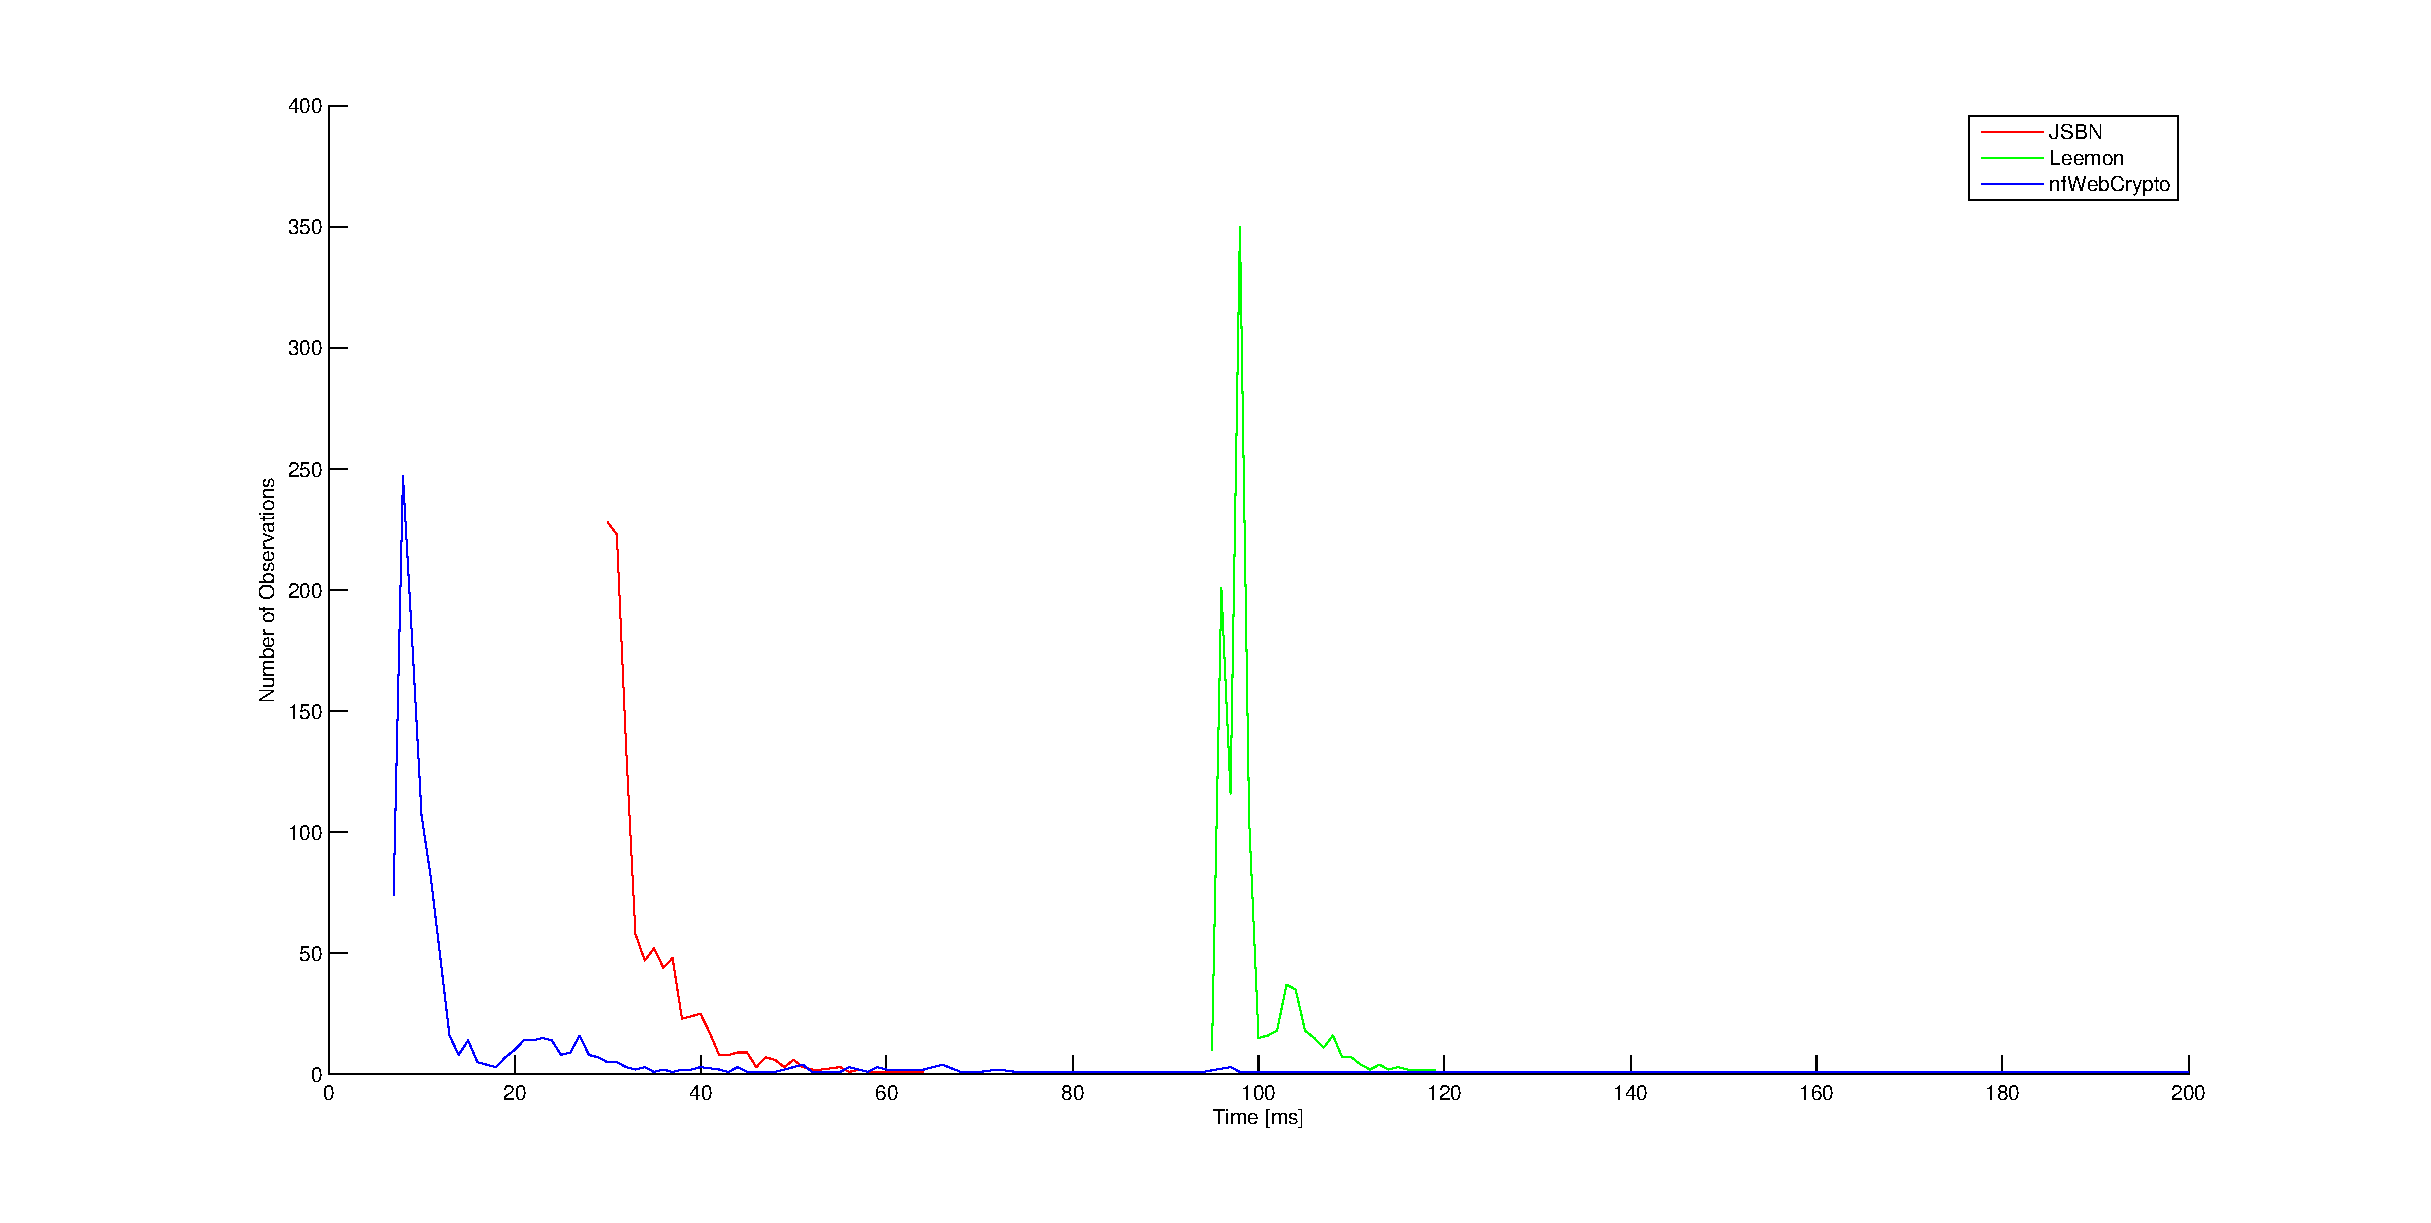
\includegraphics[width=\linewidth]{wc/modular_exponentiation.eps}
  \caption{Modulaire exponentiatie}
  \label{fig:wc:modular_exponentiation}
\end{figure}

\begin{table}
  \centering
  \caption{Modulaire exponentiatie}
  \label{tab:wc:modular_exponentiation}
  \begin{tabular}{r | c c}
    Library & Gemiddelde [ms] & Variantie [ms] \\ \hline
    JSBN & 33,9250 & 26,5019  \\
    Leemon & 99,1470 & 15,0785 \\
    NfWebCrypto & 16,0670 & 470,6251
  \end{tabular}
\end{table}

\subsubsection{RSA}

Een tweede vergelijking werd gemaakt tussen JSBN en NfWebCrypto voor een RSA encryptie. Dit wordt niet gebruikt in Helios, maar ook deze resultaten zijn zeer interessant. De berekening van de RSA cijfertekst is opnieuw een modulaire exponentiatie (\ref{eq:wc:rsa}).\cite{rivest_shamir_adleman_rsa}

\begin{equation}
  \label{eq:wc:rsa}
  c = m^e \mod{n}
\end{equation}

\npar Hier is het paar $(n, e)$ de publieke sleutel van de partij waarvoor het bericht ge\"encrypteerd wordt. Voor de publieke exponent $e$ werd de standaardwaarde \np{65537} genomen. Merk op dat deze heel wat korter is dan de \np{1024}-bit exponenten die in de tests van \ref{sec:wc:modulaire_exponentiatie} gebruikt werden. De lengte van de modulus is \np{1024} bit.

\npar De JSBN library voorziet in enkele klassen specifiek voor RSA encryptie en decryptie. Het is dus zeer eenvoudig om een bepaalde klaartekst te encrypteren met een gegeven publieke sleutel. De Web Cryptography API ondersteunt hiervoor het \texttt{RSAES-PKCS1-v1\_5} algoritme.\cite{rfc3447} Hoewel het mogelijk zou moeten zijn om publieke sleutels in het SPKI-formaat te importeren, bleek het opnieuw moeilijk om de sleutel die gebruikt werd voor de JSBN encryptie om te zetten. Daarom werd besloten om voor elke encryptie een nieuwe sleutel te genereren. De tijd die hiervoor nodig is, wordt niet meegerekend in het eindresultaat.

\npar Ook hier werd de encryptie \np{1000} keer uitgevoerd. De resultaten van deze test zijn terug te vinden in \ref{fig:wc:rsa} en \ref{tab:wc:rsa}. We zien dat de JavaScript implementatie voor deze veel kortere exponent sneller is dan de berekening door de NfWebCrypto plugin. De communicatie met de plugin weegt hier duidelijk zwaarder door.

\begin{figure}
  \centering
  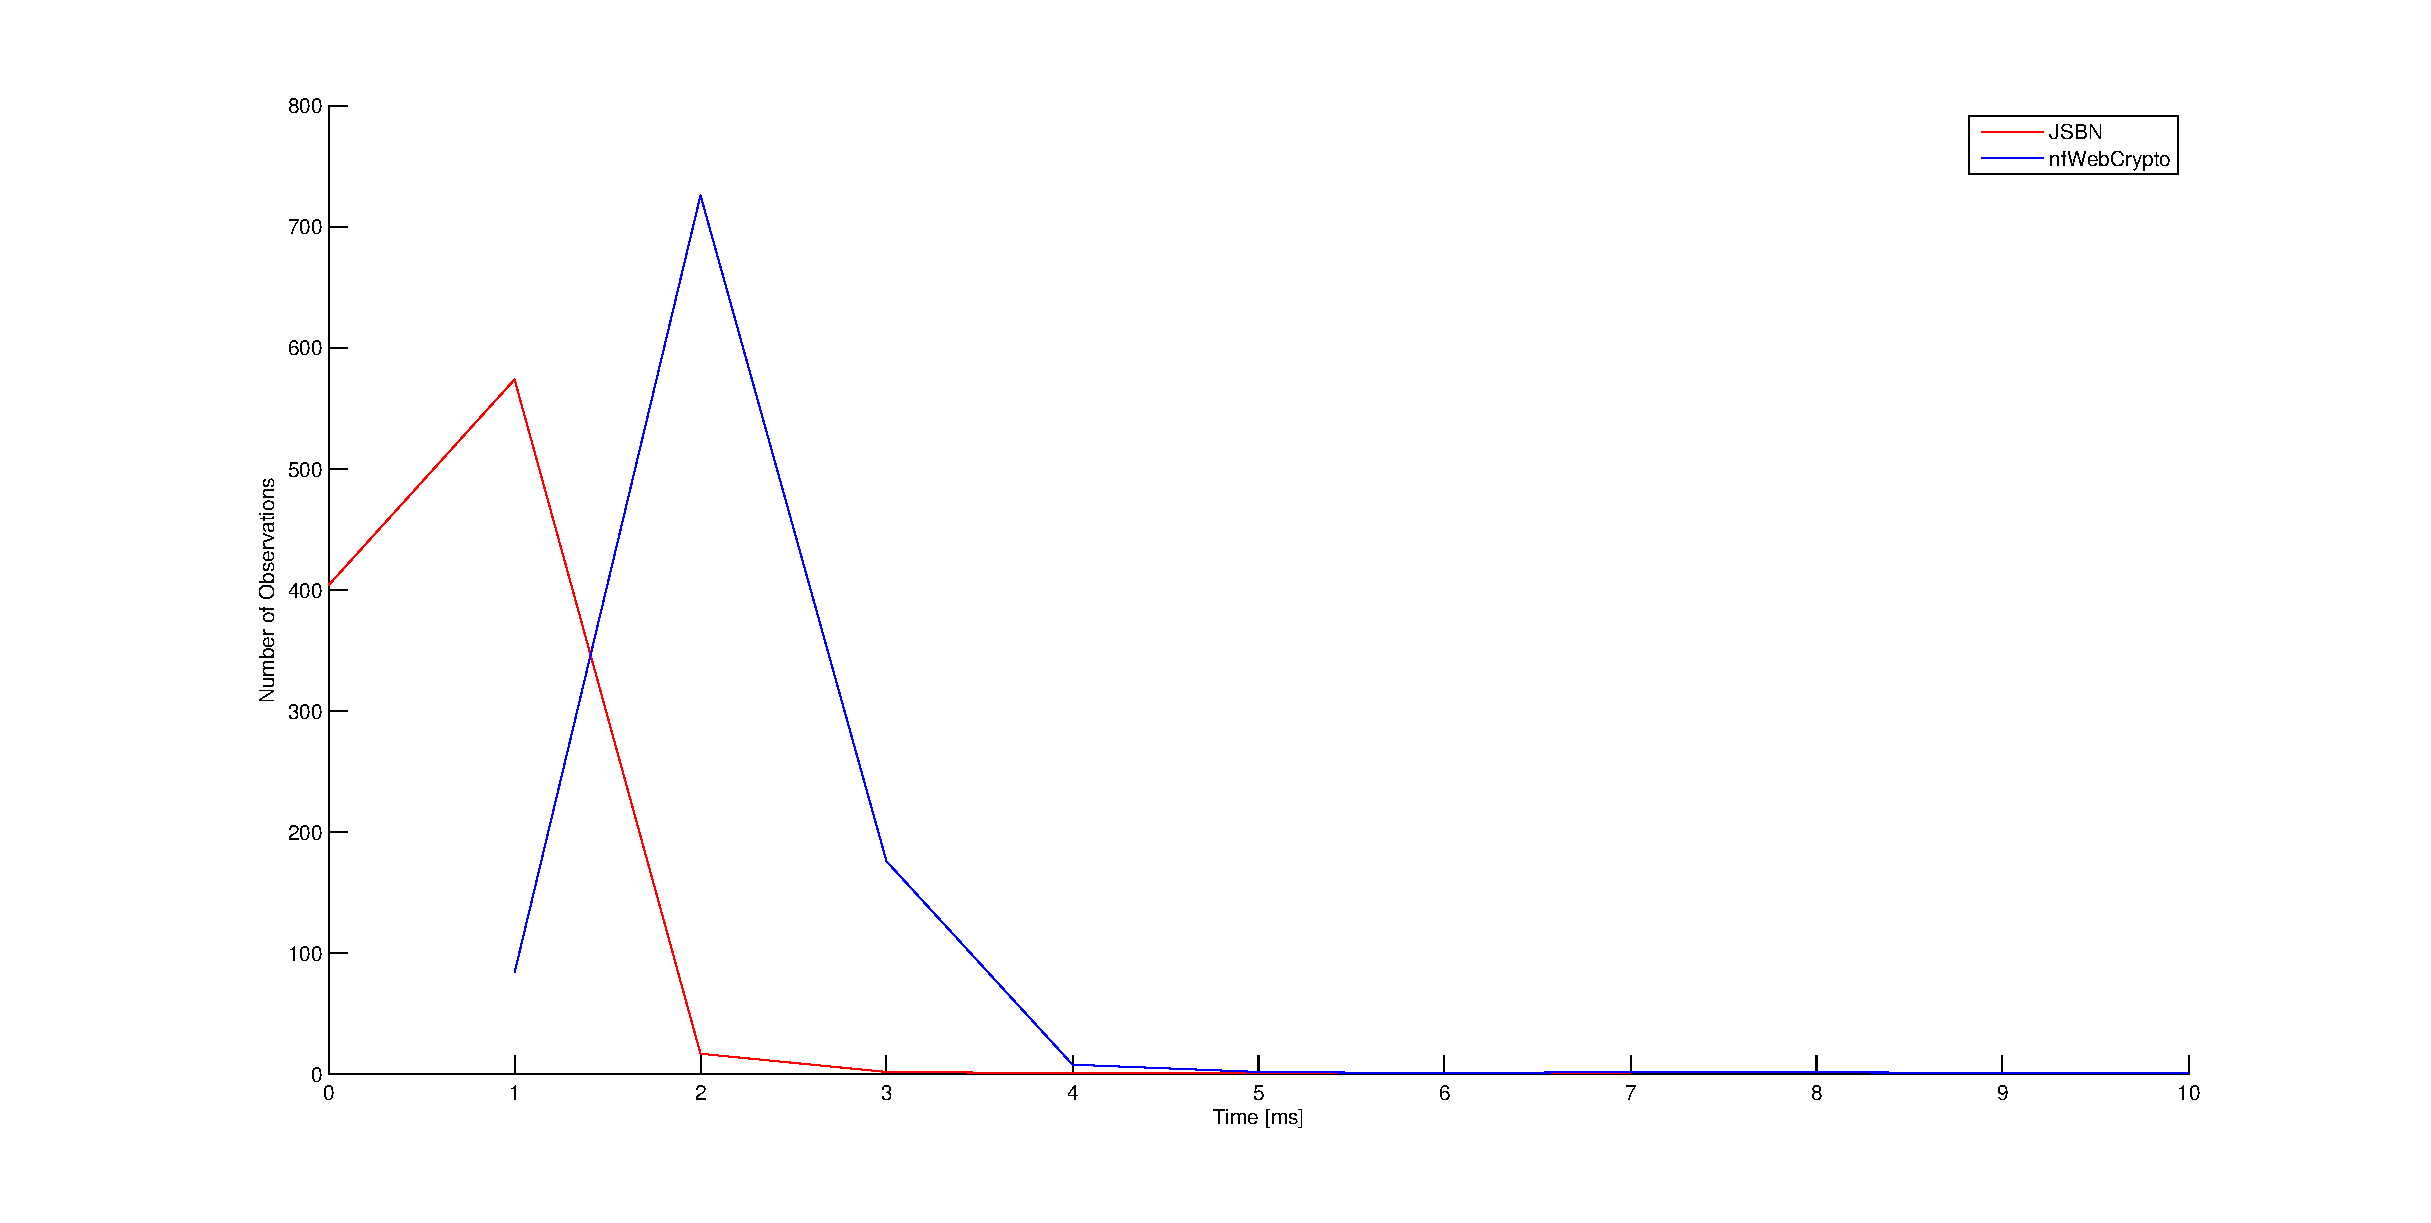
\includegraphics[width=\linewidth]{wc/rsa.eps}
  \caption{RSA}
  \label{fig:wc:rsa}
\end{figure}

\begin{table}
  \centering
  \caption{RSA}
  \label{tab:wc:rsa}
  \begin{tabular}{r | c c}
    Library & Gemiddelde [ms] & Variantie [ms] \\ \hline
    JSBN & 0,6310 & 0,3632  \\
    NfWebCrypto & 2,1360 & 0,4219
  \end{tabular}
\end{table}

\section{Besluit}

Dankzij de Web Cryptography API zal het eenvoudiger worden om cryptografie te gebruiken in de browser. Bovendien is er een merkbare snelheidswinst ten opzichte van de huidige JavaScript implementaties, wat belangrijk is voor de gebruiksvriendelijkheid. 

\npar Dat slechts een beperkt aantal algoritmes ondersteund wordt, is een belangrijk nadeel van de API. Omdat de methodes die publiek beschikbaar zijn op een hoog niveau werken, is het zeer moeilijk om deze te gebruiken voor het versnellen van alternatieve algoritmes.

\npar Daarnaast was het ook ingewikkeld om sleutels die buiten de plugin gegenereerd waren, correct te importeren. Dit werd echter voornamelijk veroorzaakt door de encoding van de communicatie en is dus niet noodzakelijk een ontwerpprobleem van de API.

  % 
% Besluit
% @author Pieter Maene <pieter.maene@student.kuleuven.be>
%

\chapter{Besluit}
\label{chap:besluit}

Om het vertrouwen van kiezers in het resultaat te vergroten, kan een voter-verifiable verkiezingssysteem gebruikt worden. Er zijn verschillende papieren systemen beschikbaar die dit realiseren, maar deze hebben zeer complexe procedures. Hierdoor kunnen ze vaak niet op grote schaal gebruikt worden in de praktijk. Helios is een voter-verifiable stemsysteem voor online verkiezingen. Dit betekent wel dat het alleen gebruikt kan worden wanneer dwang geen grote bedreiging vormt.

\npar De procedure die gevolgd moet worden om een verkiezing op te zetten in de aangepaste versie van Helios werd besproken. De interface werd ook zo aangepast dat deze procedure er veel duidelijker in terug te vinden is. In de praktische tests bleek dat deze nieuwe interface een grote hulp was. Beheerders van de verkiezing konden zonder veel aanwijzingen een verkiezing met threshold encryptie opzetten.

\npar Om Helios te gebruiken in de kringverkiezing van VTK, werden eerst nog enkele aanpassingen doorgevoerd. Vervolgens werd alles grondig getest en op basis van de gegeven feedback nog verder gewijzigd. Vooral de procedure in het stemhokje werd tijdens deze tests als te complex ervaren. Het gewijzigde systeem werd tenslotte gebruikt bij een echte verkiezing, waarbij geen grote problemen vastgesteld werden. Er kwamen ook geen klachten over het systeem.

\npar Tot slot werden twee mogelijke toekomstige uitbreidingen besproken. Ten eerste werden aanbevelingen gedaan voor het bewaren van geheime sleutels en fingerprints. De geheime sleutels van de trustees worden bewaard in een bestand. Om de sleutels te beveiligen kan ofwel de partitie ge\"encrypteerd worden, ofwel de bestanden zelf. Als alternatief zouden deze ook in de browser zelf opgeslagen kunnen worden. Visuele hashes zouden het bewaren en vergelijken van de fingerprints sterk vergemakkelijken.

\npar Ten tweede werden de prestaties van de Web Cryptography API onderzocht. Deze geeft web ontwikkelaars eenvoudig toegang tot cryptografische functies. Uit de vergelijkingen met bestaande JavaScript implementaties bleek dat deze ook een grote snelheidsverbetering opleveren. Er wordt wel slechts een beperkt aantal algoritmes ondersteund en de API biedt alleen high-level functies aan, waardoor het zeer moeilijk is om alternatieven te implementeren.


  \appendix
  
  \chapter{English Paper}
  \includepdf[pages={-}]{../Paper/paper.pdf}

  \backmatter

  % Bibliography
  \nocite{*}

  \bibliographystyle{plain}
  \bibliography{references}

\end{document}